\section{Propositional Logic}

Logic can most simply be broken down into statements. If a statement has a definitive \it{TRUE} or \it{FALSE} value, then the statement is called a \bf{proposition}. \\


\subsection{Logical Operators}

If we suppose that $p,q,r,s$ can be any propositional statement that could be either true or false, then we can build \it{truth tables} though the use of various \bf{logical operators} which are explained below:

\begin{itemize}
    \item \bf{NEGATION $\neg$:} Pronounced "not $p$"; takes the opposite value of whatever $p$ is. This is a \it{unitary operator} because it acts on only one proposition
    \item \bf{CONJUNCTION $\wedge$:} Pronounced "$p$ and $q$; this is true when both $p$ and $q$ are true and false in every other instance
    \item \bf{DISJUNCTION $\vee$:} Prononced "$p$ or $q$"; this is true when either $p$ or $q$ are true and false in every other instance (an easier way to remember this is that the disjunction is false when both $p$ and $q$ are false and true in every other instance)
    \item \bf{EXCLUSIVE OR $\oplus$:} Pronounced "$p$ or $q$, but not both"; this is true when $p$ and $q$ have opposite vales and false when they have the same value
    \item \bf{CONDITIONAL STATEMENT $\rightarrow$:} Pronounced "If $p$ then $q$"; this statement is false when $p$ is true and $q$ is false and true in all other cases 
    \item \bf{BICONDITIONAL STATEMENTS $\leftrightarrow$:} Pronounced "$p$ if and only if $q$", this is true when $p$ and $q$ have the same truth values and false in all other cases
\end{itemize}

The following are the truth tables for each of the logical operators described above:\\



\subsection{Types of Conditional Statements}

A conditional statement can take on many different forms. If $p \rightarrow q$ is the original conditional statement, then the following are variations of this statement:

\begin{itemize}
    \item \bf{CONVERSE:} $q \rightarrow p$
    \item \bf{CONTRAPOSITIVE:} $\neg q \rightarrow \neg p$
    \item \bf{INVERSE:} $\neg p \rightarrow \neg q$
\end{itemize}

\bf{INSERT A PROBLEM ABOUT THIS HERE}

\bf{INSERT TRUTH TABLES FOR ALL 4 OF THESE HERE}


\subsection{Bitwise Operations}

If we say that TRUE = 1 and FALSE = 0, then we can use bit strings to represent sets of propositions. To do bitwise operation on these, simply perform the operation on each corresponding bit in the same position.\\

\bf{INSERT PROBLEM WITH BIWISE OPERATION HERE}



\section{Propositional Equivalences}

\begin{definition}{def1.2.1:label}
    A compound proposition $r$ that is always true regardless of the truth values of the individual propositions is called a \bf{tautology}, written as $r \equiv T$.\\

    A compound proposition $r$ that is always false regardless of the truth values of the individual propositions is called a \bf{contradiction}, written as $r \equiv T$.\\

    A compound proposition $r$ that is neither a tautology nor a contradiction is called a bf{contingency}.
\end{definition}

\begin{definition}{def1.2.2:label}
    Two compound propositional statements $r$ and $s$ that have identical truth columns are called \bf{logically equivalent} and are written as $r \equiv s$.
\end{definition}


\begin{center}
    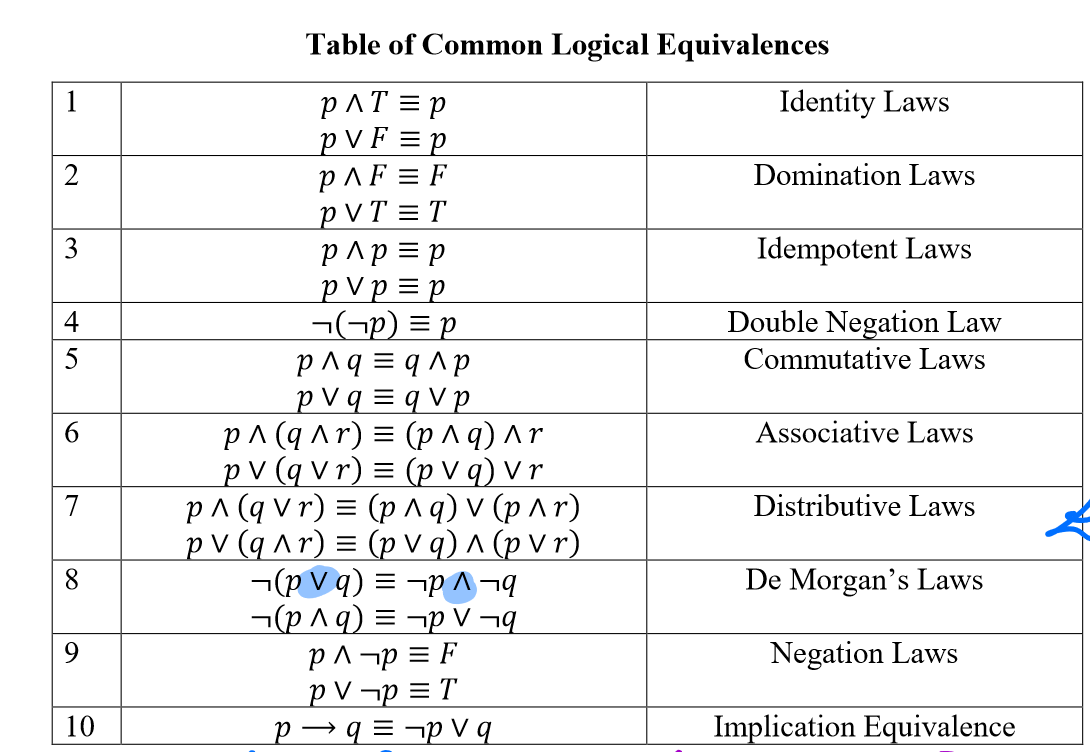
\includegraphics[width=0.75\textwidth]{chapters/ch1/images/fig1.2.1.PNG}
\end{center}



\section{Predicates and Quantifiers}

Before we dive into this section, it is important to be on the same page in terms of some common notation:

\begin{itemize}
    \item The natural numbers: $\N = \{0,1,2,3,4,\dots\}$
    \item The integers: $\Z = \{\dots -2, -1, 0, 1, 2, \dots\}$
    \item the positive integers: $\Z^+ = \{1,2,3,4,\dots\}$
    \item the rational numbers: $\Q = \{\frac{a}{b} | a, b $ are integers where $ b \ne 0\}$
    \item the real numbers: $\R = (-\infty, \infty)$
    \item the positive real numebrs: $\R^+ = (0, \infty)$
    \item the complex numbers: $\C = \{a+bi | a,b $ are real numbers$\}$
\end{itemize}